\usetikzlibrary{calc}
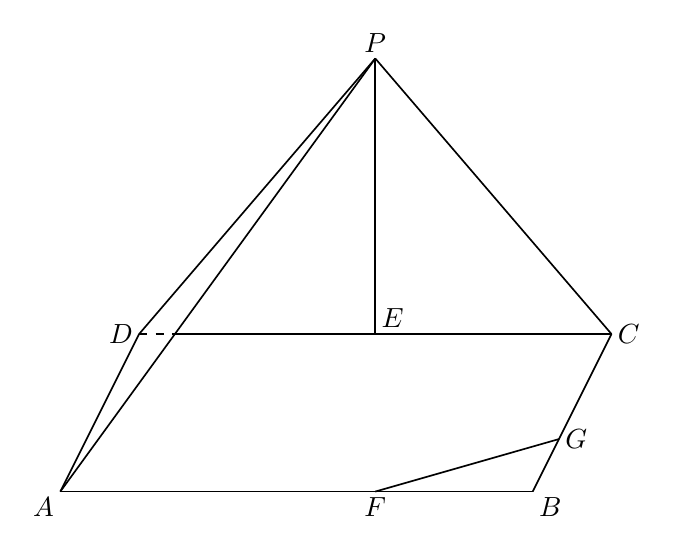
\begin{tikzpicture}[x=1cm,y=1cm,line width=0.6pt]
  \coordinate (P) at (3.0,5.5);
  \coordinate (D) at (0.0,2.0);
  \coordinate (C) at (6.0,2.0);
  \coordinate (A) at (-1.0,0.0);
  \coordinate (B) at (5.0,0.0);
  \coordinate (X) at (0.454545,2.0);
  \coordinate (E) at (3.0,2.0);
  \coordinate (F) at (3.0,0.0);
  \coordinate (G) at (5.3333,0.6667);
  \draw (A) -- (B);
  \draw (B) -- (C);
  \draw[dashed] (D) -- (X);
  \draw (X) -- (C);
  \draw (A) -- (D);
  \draw (P) -- (D);
  \draw (P) -- (A);
  \draw (P) -- (C);
  \draw (P) -- (E);
  \draw (F) -- (G);
  \node[above,inner sep=2pt] at (P) {$P$};
  \node[left,inner sep=2pt] at (D) {$D$};
  \node[above right,inner sep=2pt] at (E) {$E$};
  \node[right,inner sep=2pt] at (C) {$C$};
  \node[below left,inner sep=2pt] at (A) {$A$};
  \node[below,inner sep=2pt] at (F) {$F$};
  \node[below right,inner sep=2pt] at (B) {$B$};
  \node[right,inner sep=2pt] at (G) {$G$};
\end{tikzpicture}
